\chapter{Elvégzett munka}


\section{Koncepció}
Állapottérképek formális verifikációjának támogatása MagicDraw-ban, egy plug-in fejlesztésével lett megvalósítva. A plug-in függ a Viatra For MagicDraw-tól, ami lehetővé teszi modellek transzformációját Viatra segítségével aminek a 2.0.1-es verziója van használva. A plug-in legfontosabb funkciója MagicDraw modellek Gamma modellekké való transzformációja. A letranszformált már Gamma nyelvű modelleket az keretrendszer kezelni tudja, a verifikáció elvégzéséhez az eszköznek csak egyes részei szükségesek (\ref{fig:used-gamma} ábra). A plug-in MagicDrawToGammának lett elnevezve.

\begin{figure}[!ht]
	\centering
	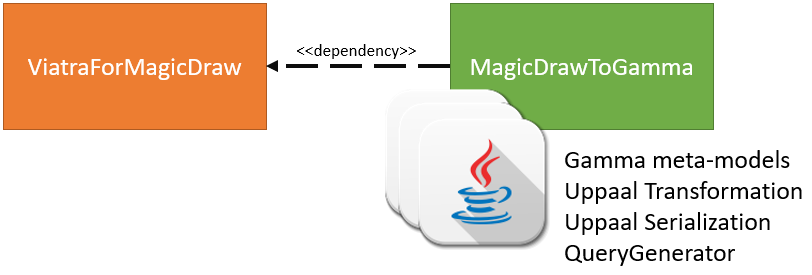
\includegraphics[keepaspectratio, width=120mm]{figures/plan.png}
	\caption{Architektúra koncepció}
	\label{fig:used-gamma}
\end{figure}

\section{Fejlesztőkörnyezet}
 A fejlesztés fejlesztő környezet előkészítésével kezdődött. MagicDraw biztosít egy ún. skeletont Eclipsehez és IntelliJhez is plug-in fejlesztéséhez, de a fejlesztés nem ezek segítségével hanem az IncQueryLabs által készített skeleton felhasználásával valósult meg. Ez már elő volt készítve V4MD használatához.
 
A skeleton egy Eclipse project, viszont Gradlet használ a projekt fordításához és a dependenciák kezeléséhez, ez sokszor inkonzisztenciákhoz vezetett, az egyik legnagyobb probléma a Viatra Querik generálása amit Gradleel nem csak Eclipsel lehet generálni. A kódbázis egy része nem Javában hanem Xtendben íródott, a Viatra trafók implementálása ezzel a nyelvvel egyszerűbb, ahol viszont nem volt indokolt ott Java 8 ban íródott az implementáció.

A dolgozat elkészítése idén a MagicDraw 19-es verziója is elérhető volt a plug-in azonban még nem ehhez, hanem a 18.5-ös verziójához íródott. A kódbázis azonban kompatibilis lehet még az újabb verziókkal is, amennyiben az állapottérképeket érintő meta-modellek nem változnak.

A Gamma dependenciák .jar fájlok formájában vannak a projekthez linkelve. Az eredeti elképzelés szerint, ahol csak lehet a Gamma nem legyen módosítva, viszont egyes részei Viatra 1.6 függőséggel bírtak ami problémákat okozott: a plug-in más verzióját használja az eszköznek, ezért az érintett részekben, az implementáció módosítva lett, hogy azok is Viatra 2-es Api-t használjanak.

A Gamma a verifikációt Uppaal segítségével végzi el, ehhez előállít egy leírást a rendszerről és egy queryt. Utóbbi megírásához biztosít egy QueryGenerátort amivel a felhasználó az Uppaal ismerete nélkül is képes a verifikálandó tulajdonságok definiálására. A QueryGenerator viszont a Gamma Eclipse plug-in részéhez tartozik ezért az implementáció módosítása itt is szükséges volt, hogy önálló részként is képes legyen működni. Ez a funkció teljesen át lett emelve Gammából módosított implementációval a MagicDrawToGammára, jelentős részben azonban az eredeti implementáció dominál.

\subsection{MagicDraw - Gamma transzformáció}
